\documentclass[a4paper]{article}

%% Language and font encodings
\usepackage[english]{babel}
\usepackage[utf8x]{inputenc}
\usepackage[T1]{fontenc}


%% Sets page size and margins
\usepackage[a4paper,top=3cm,bottom=2cm,left=3cm,right=3cm,marginparwidth=1.75cm]{geometry}

%% Useful packages
\usepackage{amsmath}
\usepackage{graphicx}
\usepackage[colorinlistoftodos]{todonotes}
\usepackage[colorlinks=true, allcolors=blue]{hyperref}


\usepackage{tikz}
\usepackage{xcolor}
%Definições para o pacote TIKZ
\definecolor{violet}{cmyk}{0.79,0.88,0,0}
\tikzstyle{state}=[draw,circle,blue, text=violet, inner sep=0pt,minimum width=30pt]            



\title{Simulação de Epidemias, 2017/1}
\author{Daniel Menasché e Vilc Rufino}

\begin{document}
\maketitle

\begin{abstract}
O  obetivo deste trabalho de simulação é introduzir conceitos básicos de um simulador de eventos discretos, e experimentar diferentes fatores que impactam na disseminação de epidemias.
\end{abstract}

\section{Introdução}

O estudo de epidemias iniciou-se há pelo menos 200 anos atrás.  Recentemente, epidemias atraem atenção não só de biólogos, mas também de cientistas das computação, tendo em vista o entendimento da disseminação de malwares como o caso recente do 
% OBS.: o HeartBleed não foi um malware, foi uma vulnerabilidade, o malware explora a vulnerabilidade
% HeartBleed\footnote{https://www.us-cert.gov/ncas/alerts/TA14-098A} e o vírus 
Wanna Crypt\footnote{https://blogs.technet.microsoft.com/mmpc/2017/05/12/wannacrypt-ransomware-worm-targets-out-of-date-systems/}.

O objetivo deste trabalho é implementar um simulador de eventos discretos que capture o efeito de diferentes parâmetros, como taxa de cura e taxa de infecção, na disseminação de um vírus.

\section{Conceitos Básicos}

Consideramos uma população finita de $N$ usuários, conectados em uma clique (todos os usuários estão conectados com todos os outros).

Cada usuário pode estar em um dentre dois estados:
\begin{enumerate}
\item \textbf{suscetível (S):} um nó no estado suscetível pode tornar-se infectado seja por conta de infecções exógenas (agente infectante fora da rede, e.g.: um pen drive) ou endógenas (agente infectante participante da rede, e.g.: um vizinho contaminado)
\item \textbf{infectado (I):} um nó infectado pode infectar seus vizinhos.  Um nó infectado torna-se limpo depois de um tempo exponencial, com taxa de descontaminação $\mu$ (tempo médio para descontaminação igual a $1/\mu$)
\end{enumerate}

Assuma que infecções exógenas chegam a cada nó segundo um fluxo Poisson com taxa $\lambda$.   

Assuma também que cada nó infectado infecta cada um de seus vizinhos segundo um fluxo Poisson com taxa $\gamma$.

A figura~\ref{fig:SISmodel} apresenta um modelo de transição de estados para um nó:

\begin{figure}[!htb]
\begin{center}
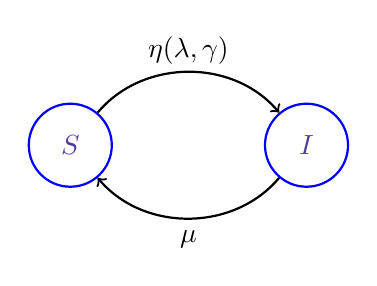
\begin{tikzpicture}[thick]%

	\begin{scope}
		\draw  (0,0)   node (State_1S) [state]  {$S$};
		\draw  (3,0)   node (State_1I) [state]  {$I$};
		
		\draw [->] (State_1S) to [out= 50 ,in= 130] (State_1I);
		\draw [->] (State_1I) to [out=-130,in= -50] (State_1S);
		
		\draw [color=black, thick] (1.5,1.2)  node{$\eta(\lambda,\gamma)$};
		\draw [color=black, thick] (1.5,-1.2)  node{$\mu$};
	\end{scope}

\end{tikzpicture}
 
\caption{Diagrama de estados para o modelo de epidêmico SIS.}
\label{fig:SISmodel}
\end{center}
\end{figure} 

onde:
\begin{table}[!htb]
\center
	\begin{tabular}{|l|l|}
    \hline
	$\mu$	&	Taxa de descontaminação (limpeza)	\\ 
    \hline
	$\eta$	&	Taxa de infecção em função das taxas exógena ($\lambda$) e endógena ($\gamma$)\\ 
    \hline
	$S$		&	Estado suscetível \\ 
    \hline
	$I$		&	Estado infectado \\
    \hline
	\end{tabular} 
\end{table}


\section{Contribuições Aditivas ou Multiplicativas}

Suponha que um nó suscetível (S) tenha $d$ vizinhos infectados (I).  Assumimos que o tempo até infecção do nó suscetível é dado por uma distribuição exponencial.
Mas qual a taxa com que o nó suscetível é infectado? Ou seja, qual a taxa da variável exponencial que caracteriza o tempo até infecção? 
\begin{enumerate}
\item modelo multiplicativo: segundo o modelo multiplicativo, a taxa de infecção é igual a $\lambda \gamma^d$, ou seja, o tempo médio até infecção é igual a $1/(\lambda \gamma^d)$
\item modelo aditivo: segundo o modelo aditivo, a taxa de infecção é igual a $\lambda + d \gamma$, ou seja, o tempo médio até infecção é igual a $1/(\lambda +d\gamma)$
\end{enumerate}

No restante deste trabalho, espera-se que você considere e implemente o modelo multiplicativo.  Foi assim que a Figura~\ref{fig:probinf} foi gerada.  Embora seja obrigatória a implementação do modelo multiplicativo, se você quiser, pode também implementar o modelo aditivo, e comparar os dois modelos.  Isso pode fazer parte, por exemplo, das suas contribuições conforme apontado na seção~\ref{sec:contribuicoes2}.

\label{sec:admul}

\section{Exemplo Ilustrativo}


\begin{figure}
\centering
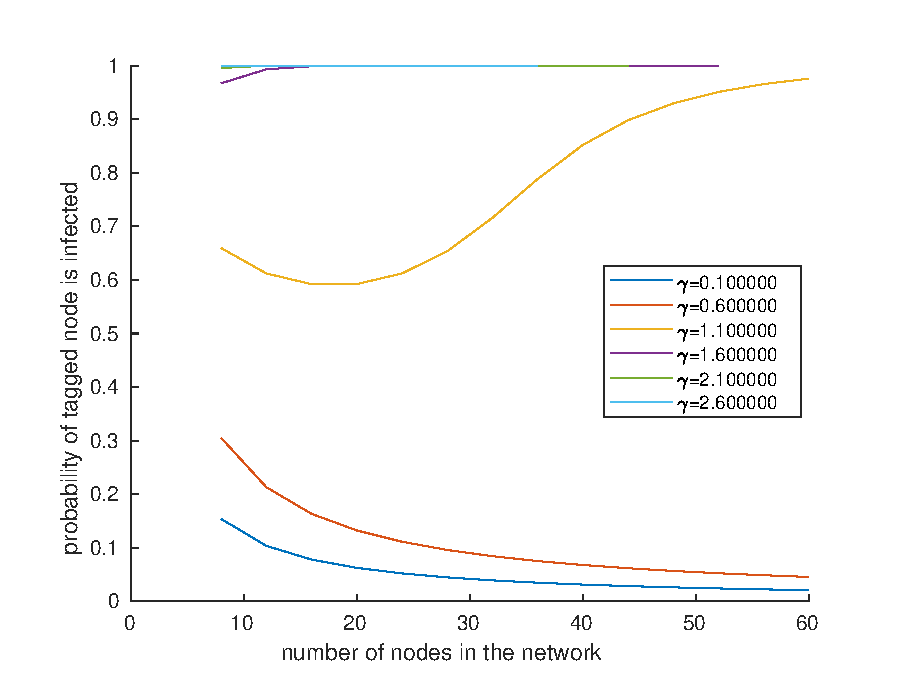
\includegraphics[width=0.8\textwidth]{epidemic_simulations.eps}
\caption{\label{fig:contamination}Probabilidade de um determinado nó estar infectado, em função do tamanho da população. A taxa de infecção endógena, $\gamma$, varia entre 0.1 e 2.6.  Para valores pequenos de $\gamma$,  a probabilidade de infecção diminui na medida em que a população aumenta.  Para valores maiores de $\gamma$, na medida em que a população aumenta a probabilidade de infecção aumenta. }
\label{fig:probinf}
\end{figure}


A Figura~\ref{fig:probinf} ilustra como a probabilidade de infecção varia em função do tamanho da população.  O tamanho da população, por sua vez, está relacionado ao número de indivíduos que não aplicaram a vacina.   Os indivíduos que tomaram a vacina estão fora de consideração, porque não podem nem se infectar, nem infectar outros nós.


Na Figura~\ref{fig:probinf} assumimos que 
infecções exógenas chegam a cada nó segundo um fluxo Poisson com taxa $\lambda=\frac{C}{N}$, onde $C$ é uma constante (definida como $1$) e $N$ é o tamanho da população (número de nós que não se vacinaram).  Note que na medida em que $N$ aumenta, a probabilidade de um nó ser infectado por um agente externo diminui.  Isso ocorre porque assumimos que o agente externo tem poder de ataque constante $C$, mas esse poder é dividido entre os $N$ membros da população.

%Logo, cada indivíduo é atacado pelo agente externo (exógeno) a taxa efetiva de $\lambda = 1/N$.

%pode aumentar ou diminuir, dependendo do valor de $\gamma$.


Seja $\pi_I$ a probabidade de um nó estar infectado.  

\textbf{Regime exógeno predominante:} Se a taxa de contaminação endógena for pequena ($0 \leq \gamma \leq 1 $), observamos que $\pi_I$ diminui na medida em que $N$ aumenta.   Isso ocorre porque nesse regime quanto maior o tamanho da população,  menor a chance de um elemento externo selecionar um determinado indivíduo como alvo. Se a população for pequena, por outro lado, existe uma grande chance de aqueles poucos indivíduos suscetíveis serem alvos fáceis do poder de contaminação do agente exógeno (e.g.: scans que buscam por elementos vulneráveis,  ZMap, que mapeia rapidamente em algumas horas vulnerabilidades em todo o espaço de endereços IPv4).  Nesse regime, o sistema é dominado por efeitos exógenos. 



\textbf{Regime endógeno predominante:} Por outro lado, quando a taxa de contaminação endógena é grande ($\gamma > 1$), observamos que $\pi_I$ aumenta na medida em que o tamanho da população aumenta.   Isso ocorre porque nesse regime, dominado por fatores endógenos, quanto mais indivíduos suscetíveis, maior a circulação do vírus na rede, e maior a chance de um nó infectar-se. Lembre que um nó infectado pode infectar seus vizinhos.


Finalmente, note que quando a taxa de contaminação endógena assume valores intermediários ($\lim_{\gamma \to 1}$), temos um comportamento híbrido (a curva de infecção primeiro diminui, e depois aumenta).

\section{Questões}

\subsection{Parte 1: Primeiros Passos}

O seu primeiro objetivo no trabalho de simulação é reproduzir a Figura~\ref{fig:probinf}.  Para tal, simule o sistema para diferentes parâmetros, e procure regerarar a Figura~\ref{fig:probinf} da forma mais fidedigna possível, incluindo intervalos de confiança.

\subsection{Parte 2: Usando a Criatividade}

\label{sec:contribuicoes2}

O segundo objetivo do trabalho é fazer variações na topologia (por exemplo, considerar uma estrela ao invés de uma clique), taxas de infecção exógena e endógena, e taxa de cura, e verificar os efeitos dessas mudanças na probabilidade de um nó estar infectado.

Você pode usar-se de sua criatividade para variar o processo de epidemia, e ver os efeitos da variação em cima dos resultados.  Uma sugestão, inclusive, foi dada na seção~\ref{sec:admul}.


\begin{table}
\center
\begin{tabular}{l|l|c}
	\hline 
	variável 	& descrição  			& valor padrão \\ 
	\hline 
	$N$ 		& tamanho da população 	& - \\
	& (número de nós não vacinados) 	& \\
	$\mu$ 		& taxa de desinfecção (cura) 		&  1 \\
	$C$			& taxa de infecção exógena agregada & 1 \\
	$\lambda = C/N$ 	& taxa de infecção exógena por nó & $1/N$\\
	$\gamma$ 	& taxa de infecção endógena & 0.1:0.5:2.6 \\
	\hline
\end{tabular}
\end{table}


\section{Trabalhos Relacioanados}


O principal trabalho relacionado a este é~\cite{zhang2014diffusion}.  É interessante que pelo menos um dos membros de cada grupo leia o trabalho relacionado, e traga ideias de como usar este trabalho relacionado para validar seu simulador, bem como para inspirar novas variantes da sua simulação que possam ser de interesse na análise.


\section{Nota}

A sua nota será proporcional a

\begin{enumerate}
\item qualidade dos seus resultados, 
\item criatividade na variação de parâmetros e cenários,
\item profundidade da discussão de resultados,
\item detalhamento das abordagens usadas para veriicação da corretude do seu simuladores, incluindo gráficos e números que comprovem que seu simulador está correto em vários casos base simples 
\end{enumerate}


\section{Dúvidas}
Dúvidas devem ser direcionadas ao Vilc (vilc@bol.com.br), de preferência com cópia para o restante da turma.


\section{Anexo}
\subsection{Modelos de epidemias}

Os métodos analíticos para modelar epidemias SIS em redes de heterogêneas por meio de suas topologias podem ser:

\begin{enumerate}
	\item  Descrição da topologia por meio de suas propriedades estatísticas como grau de distribuição e grau de correlações. Esses métodos consideram o processo de difusão no limite de grandes redes usando análise mean-field \cite{barthelemy2008dynamical}, \cite{danon2011networks}, \cite{santos2011emergent}, \cite{house2011insights} e \cite{pastor2001epidemic}; 

	\item Descrição exata da topologia por sua matriz de adjacência da rede (grafo) em análise, o qual é estático e de tamanho finito. A epidemia é tratada como um processo de Markov e a taxa de infecção é dependente do número de vizinhos infectados  \cite{draief2006thresholds}, \cite{ganesh2005effect}, \cite{chakrabarti2008epidemic}, \cite{wang2003epidemic}, \cite{zhang2012accounting};
    
\end{enumerate}

\subsubsection{Representação multiplicativa}
Uma forma de representar o processo de Markov na topologia exata é demonstrado por \cite{zhang2015contact} and \cite{zhang2014diffusion}, denominado processo \textit{scaled SIS}, onde o tempo que o nó está no estado suscetível, $\hat{T}$, é uma variável aleatória dada por uma distribuição exponencial, escalonada pela taxa de infecção exógena, $\hat{T} \sim \exp(\lambda\gamma^{d})$, onde $\lambda$ é a taxa de infecção exógena, $\gamma^{d}$ é a taxa de infecção endógena e $d$ é o número de vizinhos infectados.

	Para o caso da representação \textit{scaled SISI} o processo de Markov é reversível, e a equação de balanceamento é dada por \cite{kelly1979reversibility}:
	
	\[
	 \pi(\boldsymbol{x}) q(\boldsymbol{x},\boldsymbol{x'}) = \pi(\boldsymbol{x'})q(\boldsymbol{x'},\boldsymbol{x}) \textrm{, } \boldsymbol{x},\boldsymbol{x'} \in \mathcal{Y}
	\]

	Para o processo \textit{scaled SIS}:
	\[
	 \pi(\boldsymbol{x}) = \frac{1}{Z} \left( \frac{\lambda}{\mu}\right)^{1^{T}\boldsymbol{x}} \gamma^{\boldsymbol{x}^{T}A\boldsymbol{x}/2} \textrm{, } \boldsymbol{x} \in \mathcal{X}
	 \label{eq:equilibriumScaledSIS}
	\]
	
	Onde $Z$ é a \textit{função de partição} (normalização) definida como:
	\[
	 Z = \sum_{\boldsymbol{x} \in \mathcal{X}} \left( \frac{\lambda}{\mu}\right)^{1^{T}\boldsymbol{x}} \gamma^{\boldsymbol{x}^{T}A\boldsymbol{x}/2}
	\]
    
    $\boldsymbol{x}$ é o vetor binário que representa os agentes contaminados;
    
    $\mathcal{X}$ é o conjunto de todos os valores possíveis de $\boldsymbol{x}$

\subsubsection{Representação aditiva}
        A forma clássica de representação, que será denominada \textit{non-scaled SIS}, considera o tempo que o nó está no estado suscetível, $\hat{T}$, como uma variável aleatória dada pelo menor valor obtido entre duas distribuições exponenciais $\alpha \sim \exp(\lambda) $ e $\beta \sim \exp(\gamma d)$:
        \[ \hat{T} = min(\alpha,\beta) \]
        
        Portanto $T \sim \exp(\lambda + \gamma d)$ 

\subsection{Material disponível no dropbox}
https://www.dropbox.com/sh/x8zwkqu35m7uc21/AADZsQ\_qPgLnzpZhOZiSZocSa?dl=0
\bibliographystyle{alpha}
\bibliography{sample}

\end{document}